\subsubsection{Part 1:}

\begin{gather*}
	Throughput=\frac{rxPackets*1000*8}{txTime} \\
	TP_{user_1}=\frac{5000*1000*8}{20} \\
	= 2000 Kbps \\
	TP_{user_2}=\frac{4999*1000*8}{20} \\
	= 1999.6 Kbps \\
\end{gather*}
\captionof{equation}{Average Throuhgput (Kbps)}

\begin{figure}[H]
	\centering
	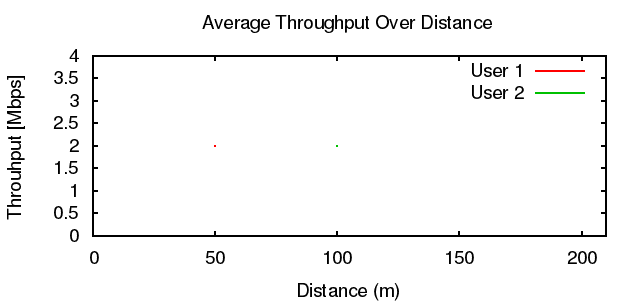
\includegraphics[width=0.8\textwidth]{images/EE500/QC/P1/Images/wifi-throughput}
	\caption{Throughput for 2 users, one at a distance of 50m, one at a
	distance of 100m}
	\label{fig:QCP1throughput}
\end{figure}

\begin{gather*}
	\overline{delay}=\frac{delaySum}{rxPackets} \\
	\overline{delay}_{user 1}=\frac{2224452124}{5000} \\
	= 444890.4248ns \\
	\overline{delay}_{user 2}=\frac{10823682785}{4999} \\
	= 2165169.591ns \\
\end{gather*}
\captionof{equation}{Average Delay (s)}

\begin{figure}[H]
	\centering
	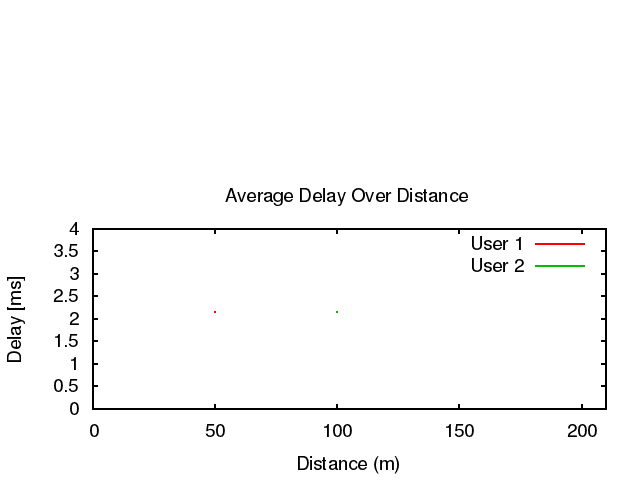
\includegraphics[width=0.8\textwidth]{images/EE500/QC/P1/Images/wifi-delay}
	\caption{Delay for 2 users, one at a distance of 50m, one at a distance
	of 100m}
	\label{fig:QCP1delay}
\end{figure}

\begin{gather*}
	PLR=\frac{lostPackets}{rxPackets+lostPackets} \\
	PLR_{user 1}=\frac{0}{5000+0} \\
	= 0 \\
	PLR_{user 2}={1}{4999+1} \\
	= 0.0002
\end{gather*}
\captionof{equation}{Average Packet Loss Ratio}

\begin{figure}[H]
	\centering
	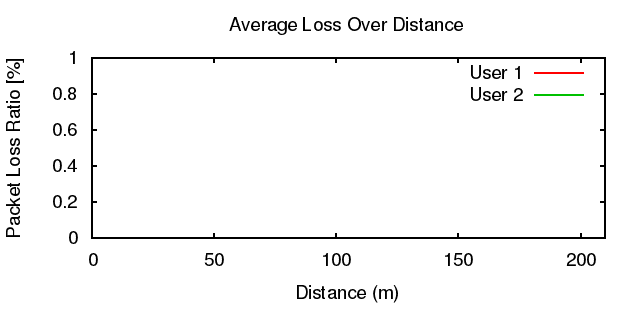
\includegraphics[width=0.8\textwidth]{images/EE500/QC/P1/Images/wifi-loss}
	\caption{Loss for 2 users, one at a distance of 50m, one at a distance
	of 100m}
	\label{fig:QCP1loss}
\end{figure}
